\documentclass[10pt]{article}

\usepackage{fancyhdr}
\usepackage{graphicx}
\usepackage{geometry}
\usepackage{lastpage}
\usepackage{titling}
\usepackage{sectsty}
\usepackage{setspace}
\usepackage{changepage}
\usepackage[shortlabels]{enumitem}
\usepackage{subcaption}
\usepackage{helvet}
\usepackage{hyperref}

\usepackage{tabularx}
\usepackage[table]{xcolor}
\usepackage{array}
\newcolumntype{P}[1]{>{\centering\arraybackslash}p{#1}}

\usepackage{siunitx}
\usepackage{nicefrac}
\usepackage{amsmath}
\usepackage{gensymb}
\usepackage{amssymb}
\usepackage{float}
\setcounter{MaxMatrixCols}{11}
\usepackage{indentfirst}

\usepackage{listings}
\usepackage{matlab-prettifier}
% \usepackage{color}
% \definecolor{dkgreen}{rgb}{0,0.6,0}
% \definecolor{gray}{rgb}{0.5,0.5,0.5}
% \definecolor{mauve}{rgb}{0.58,0,0.82}

\lstset
{
  frame=tb,
  style=Matlab-editor,
  % language=MATLAB, %Matlab-editor,
  aboveskip=3mm,
  belowskip=3mm,
  showstringspaces=false,
  columns=flexible,
  basicstyle={\small\ttfamily},
  numbers=none,
  % numberstyle=\tiny\color{gray},
  % keywordstyle=\color{blue},
  % commentstyle=\color{dkgreen},
  % stringstyle=\color{mauve},
  breaklines=true,
  breakatwhitespace=true,
  tabsize=3
}

\geometry
{
  letterpaper, 
  total={175.9mm,229.4mm}, 
  top=25mm, 
  left=20mm, 
  headheight=15pt,
  voffset=12pt,
  footskip=15pt
}
\author{Daniel Sturdivant}
\title{Homework 4}
\date{April 2023}
\graphicspath{ {./media/} }

\pagestyle{fancy}
\fancyhead[R]{April 17, 2023}
\fancyhead[L]{Sturdivant, Daniel}
\fancyhead[C]{MECH 6970 GPS}
\fancyfoot[C]{Page \thepage\ of \pageref{LastPage}}

\makeatletter
\def\@maketitle
{
  \null
  \begin{center}
    {\huge \@title \\}
  \end{center}
  \vskip 5mm
}
\makeatother

\sectionfont{\fontsize{16}{16}}
\subsectionfont{\fontsize{13}{13}\normalfont}
\renewcommand{\thesubsection}{\arabic{section}-\arabic{subsection}}
\renewcommand{\familydefault}{\sfdefault}
\newcommand{\solution}{\textbf{Solution: \\}}


%% ====================================================================== %%
\begin{document}

\maketitle
\thispagestyle{fancy}
\setstretch{1.25}
% \setlength{\parskip}{0em}
% \setlength{\abovedisplayskip}{-8pt}
% \setlength{\belowdisplayskip}{12pt}
\setlength{\parindent}{0pt}

\begin{enumerate}[label=\textbf{\arabic*.}]
  \itemsep 24pt
  
  % PROBLEM 1
  \item Write a controller (matlab or Simulink) for a simple $\dfrac{1}{s}$ 
  plant. Assume a unit step input for the reference, r(t).
  \begin{enumerate}[(a)]
    \itemsep -2pt
    \item What type of controller did you use. Provide the Gain Margin, Phase 
    Margin, closed-loop eigenvalues, and steady state error.
    \item What is the steady state error if the reference r(t) is a unit ramp 
    input?
    \item Redesign the controller to track the ramp input and repeat 
    \emph{part a}.
  \end{enumerate}
  \solution
  A proportional-integral (PI) controller was used for each part of this 
  problem. The controller was designed to be under damped with a 1 second time 
  to steady-state. Assuming, $t_{ss} = 1$ and $\zeta = 0.7071$, the controller 
  gains were determined in \emph{Equation \ref{eq:1}}.
  \begin{equation}
    \begin{split}
      \omega &= \dfrac{4.6}{\zeta t_{ss}} = 6.5054 \\
      K_i &= \omega^2 = 42.32 \\
      K_p &= 2 \zeta \omega = 9.2
    \end{split}
    \label{eq:1}
  \end{equation}
  The addition of integral control to an integrator plant makes our system Type 
  II, and therefore has zero steady-state error for both a step input or a ramp 
  input. The outputs of both scenarios are shown in \emph{Figure \ref{fig:1}}.
  \begin{figure}[H]
    \centering
    \begin{subfigure}{0.5\textwidth}
      \centering
      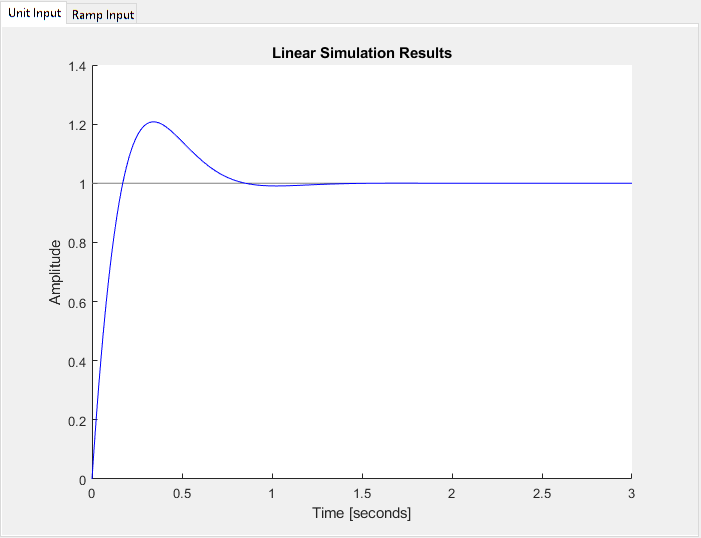
\includegraphics[width=0.95\textwidth]{p1_step.png}
    \end{subfigure}%
    \begin{subfigure}{0.5\textwidth}
      \centering
      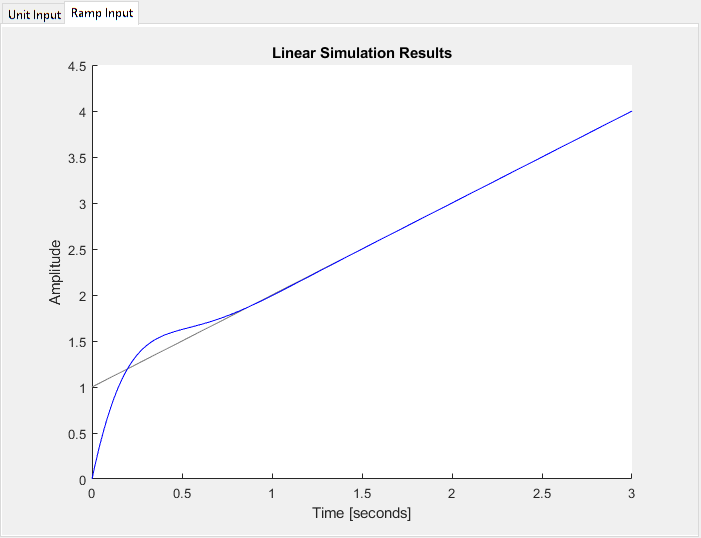
\includegraphics[width=0.95\textwidth]{p1_ramp.png}
    \end{subfigure}%
    \caption{Simulation of Step and Ramp Input on Designed System.}
    \label{fig:1}
  \end{figure}
  Using the closed-loop transfer function (\emph{Equation \ref{eq:2}}):
  \begin{equation}
    G(s) = \dfrac{9.2s + 42.32}{s^2 + 9.2s + 42.32}
    \label{eq:2}
  \end{equation}
  MATLAB's \emph{eig} and \emph{margin} functions can be used to determine the 
  closed-loop eigenvalues as well as gain and phase margin, \emph{Equation 
  \ref{eq:3}} and \emph{Figure \ref{fig:2}}.
  \begin{equation}
    s = -4.6 \pm 4.6i
    \label{eq:3}
  \end{equation}
  \begin{figure}[H]
    \centering
    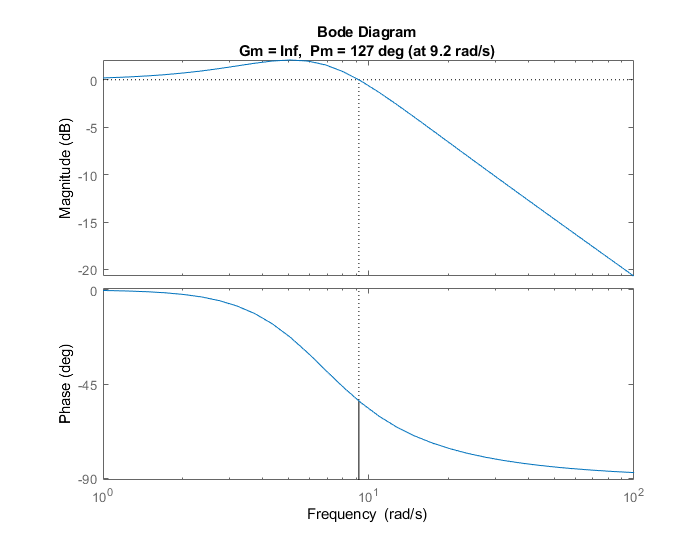
\includegraphics[width=0.6\textwidth]{p1_bode.png}
    \caption{Gain and Phase Margin of Closed Loop System.}
    \label{fig:2}
  \end{figure}
  \vspace{12pt}

  
  % PROBLEM 2
  \item Take the sampled 100 Hz sine wave (generate\_signal(1)) from the website 
  (sampled at 1 MHz, i.e. Ts=1e-6).
  \begin{enumerate}[(a)]
    \itemsep -2pt
    \item Develop a simple (1 Hz) PLL to track the phase of the signal. Provide 
    plots of phase, phase error, as well as the estimated signal vs. true signal.
    \item Double the PLL bandwidth and repeat \emph{part a}.
    \item Determine the true frequency and repeat \emph{part a}.
    \item Modify your PLL to work from the unknown frequency and repeat part a 
    assuming 10 Hz signal.
  \end{enumerate}
  \solution
  To create a controller with a bandwidth of 1 Hz, $\zeta=0.7071$,  $BW = 1$ 
  and open loop gain of $K = 4$ were chosen. Using \emph{equation \ref{eq:4}}, 
  the controller values were determined:
  \begin{equation}
    \begin{split}
      \omega &= \dfrac{4 BW \zeta}{1+\zeta^2} \\
      K_i &= \omega ^2 \\
      K_p &= \zeta \omega \\
    \end{split}
  \end{equation}
  The following code was used for the PLL and costas loops. 
  \begin{lstlisting}
  for i = 2:length(loop)
    % data signal
    sig = signal(beg:fin);
    % Inphase and Quadrature
    ssig = sin(2*pi*f(i-1).*t' + theta(i-1));
    csig = cos(2*pi*f(i-1).*t' + theta(i-1));
    I(i) = sig * ssig;
    Q(i) = sig * csig;
    % error
    disc(i) = atan(Q(i) / I(i));
    % propagate
    f(i) = f(i-1) + K * (Ki*t_int*disc(i) + Kp*(disc(i) - disc(i-1)));
    theta(i) = rem(theta(i-1) + 2*pi*f(i-1)*t_int, 2*pi);
    beg = beg + numSamp;
    fin = fin + numSamp;
  end
  \end{lstlisting}
  \emph{Figure \ref{fig:3}} contains the outputs of the PLL for \emph{part a}. 
  As shown, the controller locks on while the frequency of the incoming signal 
  is 100 Hz. As soon as the frequency changes, the controller is no longer able 
  to track the signal completely and ends up oscillating wildly around a 
  frequency of 110 Hz.
  \begin{figure}[H]
    \centering
    \begin{subfigure}{\textwidth}
      \centering
      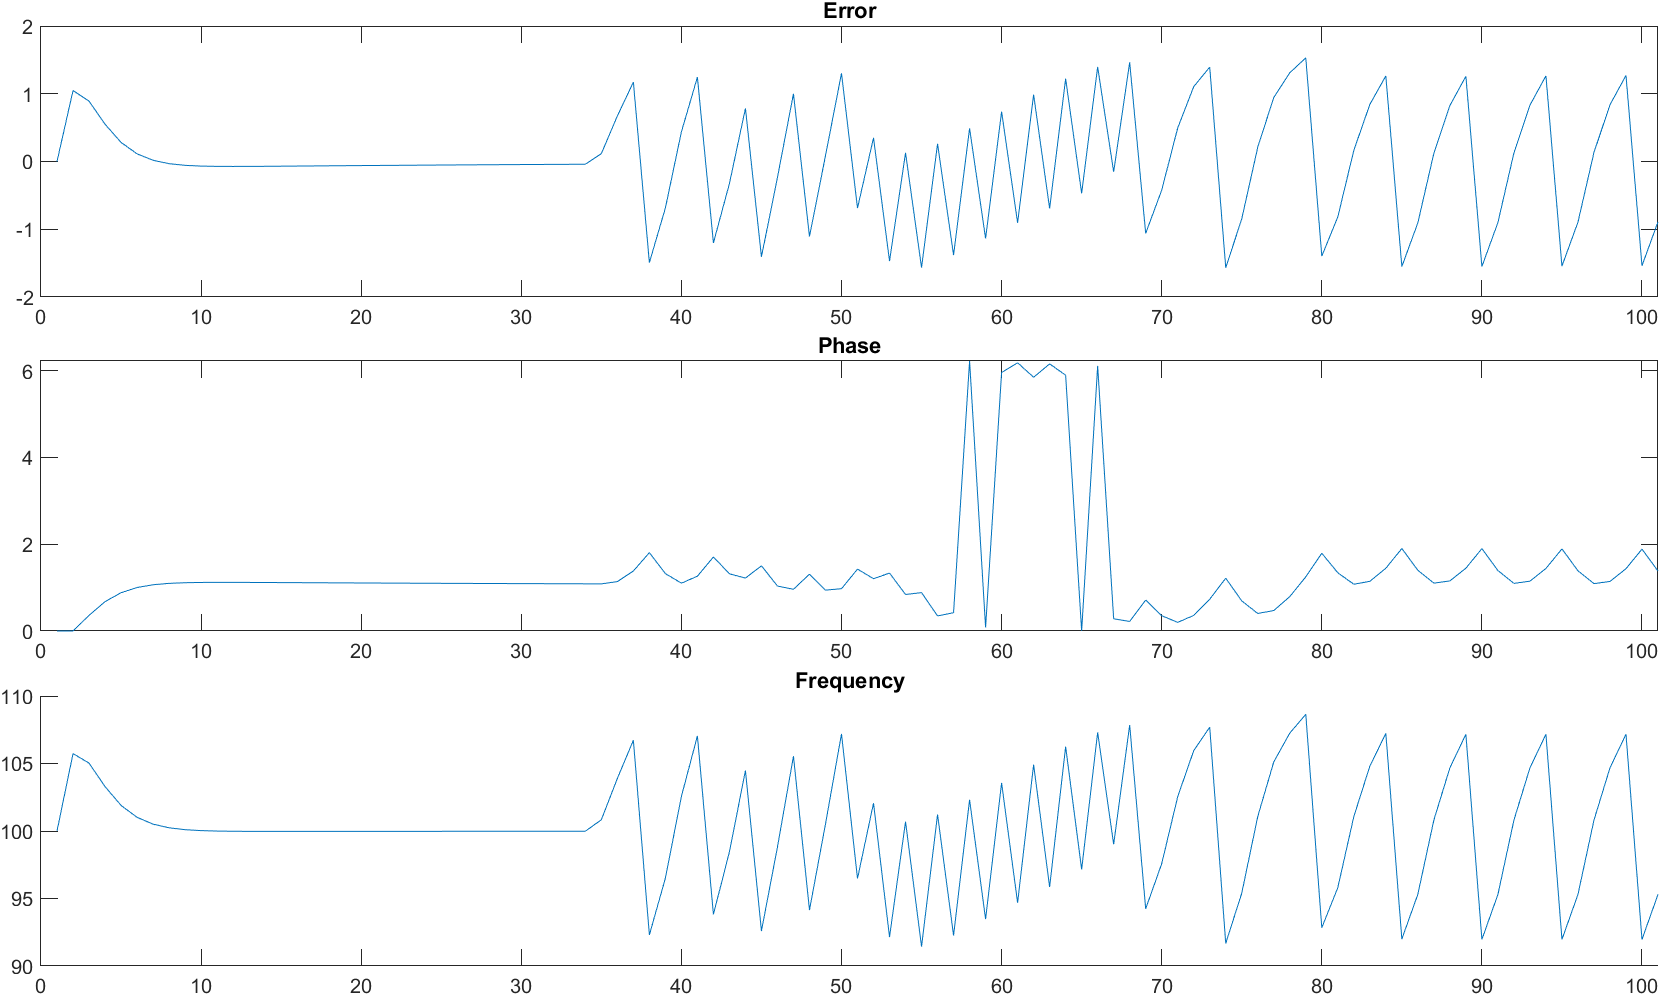
\includegraphics[width=0.7\textwidth]{p2_a.png}
    \end{subfigure}% 
    \\
    \begin{subfigure}{\textwidth}
      \centering
      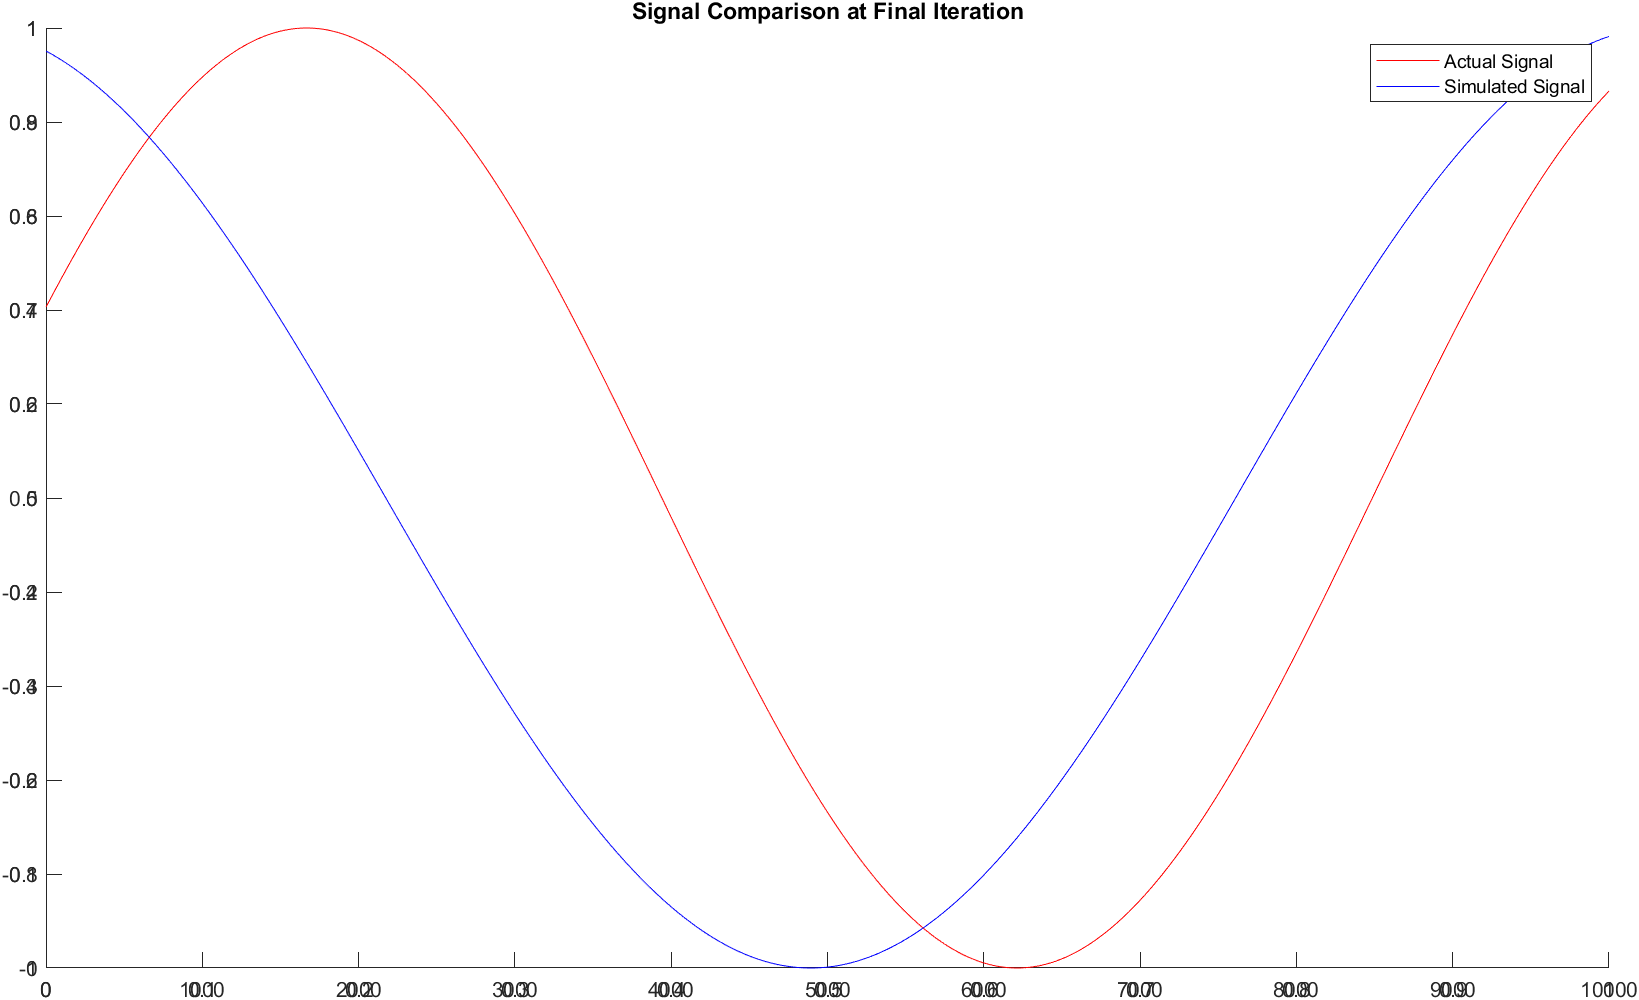
\includegraphics[width=0.7\textwidth]{p2_a_wave.png}
    \end{subfigure}%
    \caption{PLL Part A.}
    \label{fig:3}
  \end{figure}
  A similar response is received when the bandwidth is doubled to 2 Hz. The only 
  difference is more initial oscillation happens, shown in 
  \emph{Figure \ref{fig:4}}. Additionally, the overshoot at 110 Hz is reduced.
  \begin{figure}[H]
    \centering
    \begin{subfigure}{\textwidth}
      \centering
      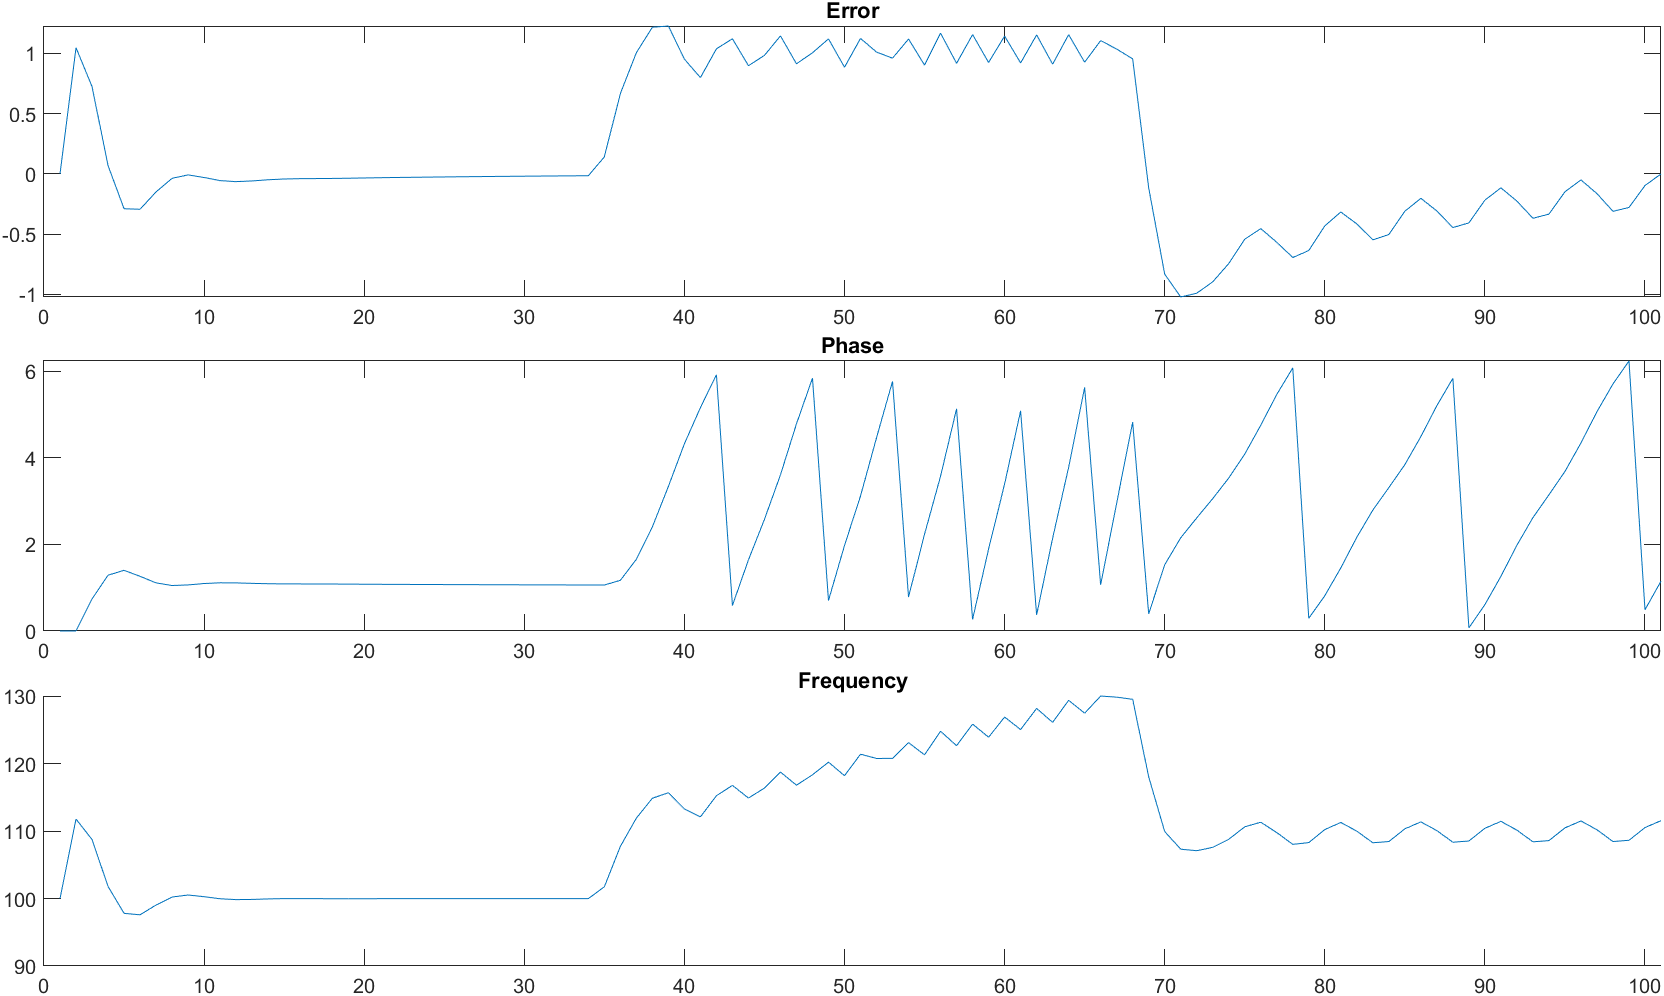
\includegraphics[width=0.7\textwidth]{p2_b.png}
    \end{subfigure}% 
    \\
    \begin{subfigure}{\textwidth}
      \centering
      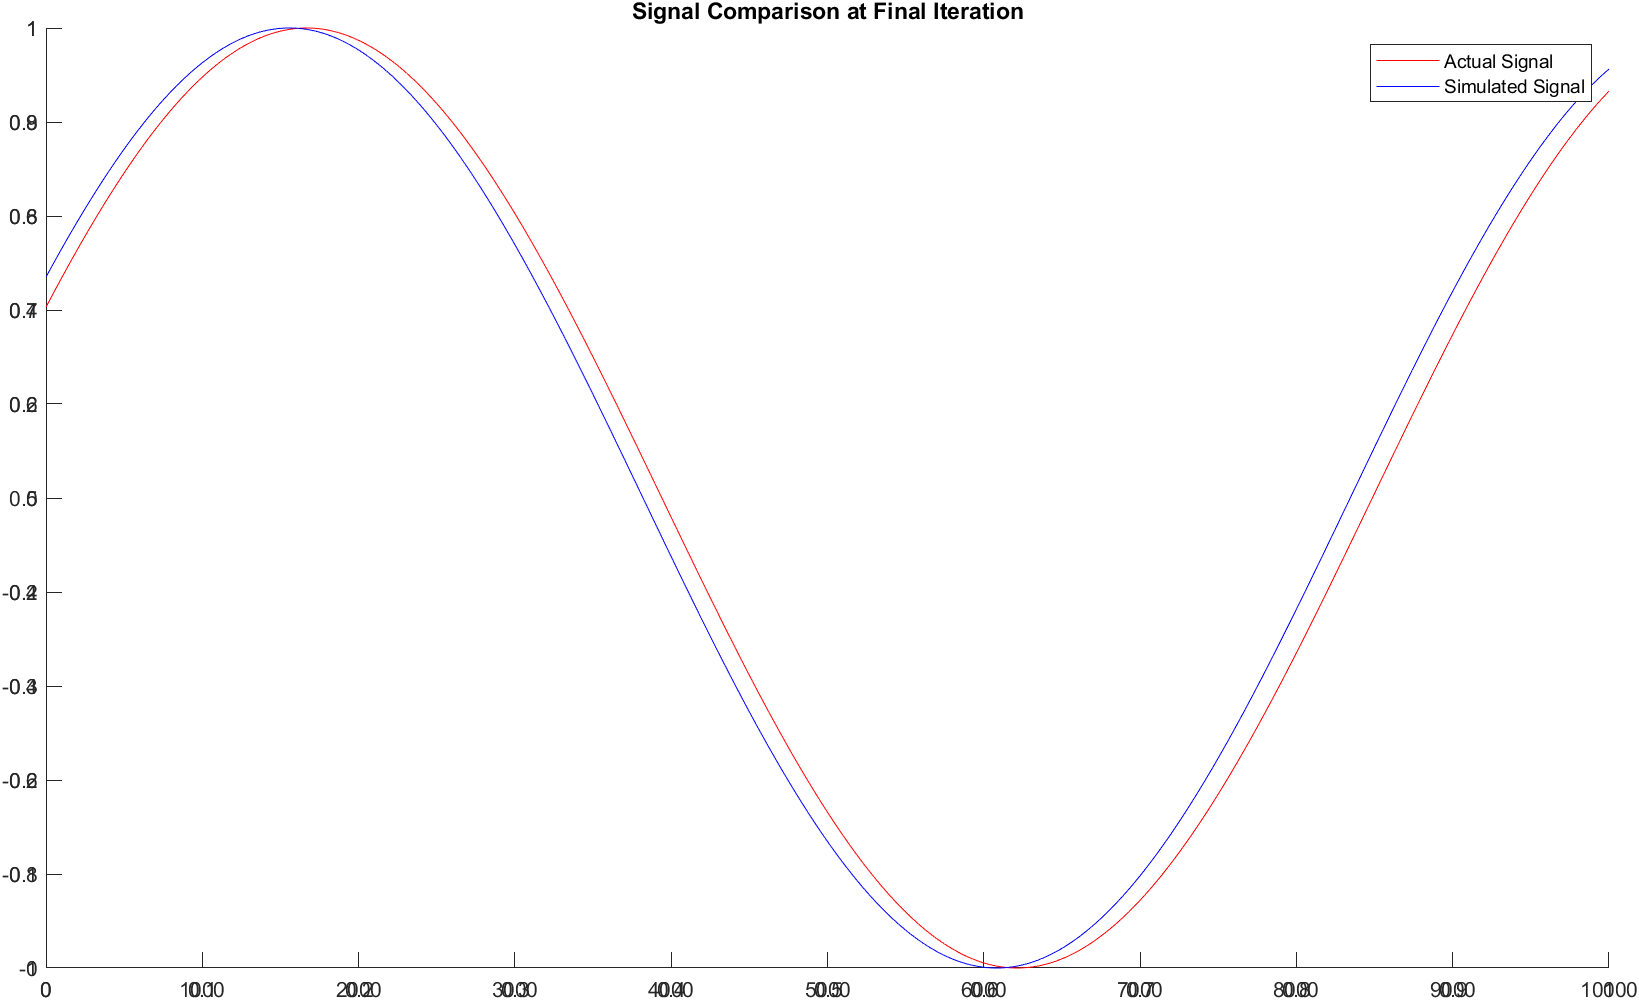
\includegraphics[width=0.7\textwidth]{p2_b_wave.png}
    \end{subfigure}%
    \caption{PLL Part B.}
    \label{fig:4}
  \end{figure}
  Switching the nominal frequency to 110 Hz instead of 100 Hz results in 
  \emph{Figure \ref{fig:5}}. There is a higher phase error magnitude, but the 
  system still converges to 100 Hz. Again the frequency change causes 
  oscillation around the 110 Hz frequency.
  \begin{figure}[H]
    \centering
    \begin{subfigure}{\textwidth}
      \centering
      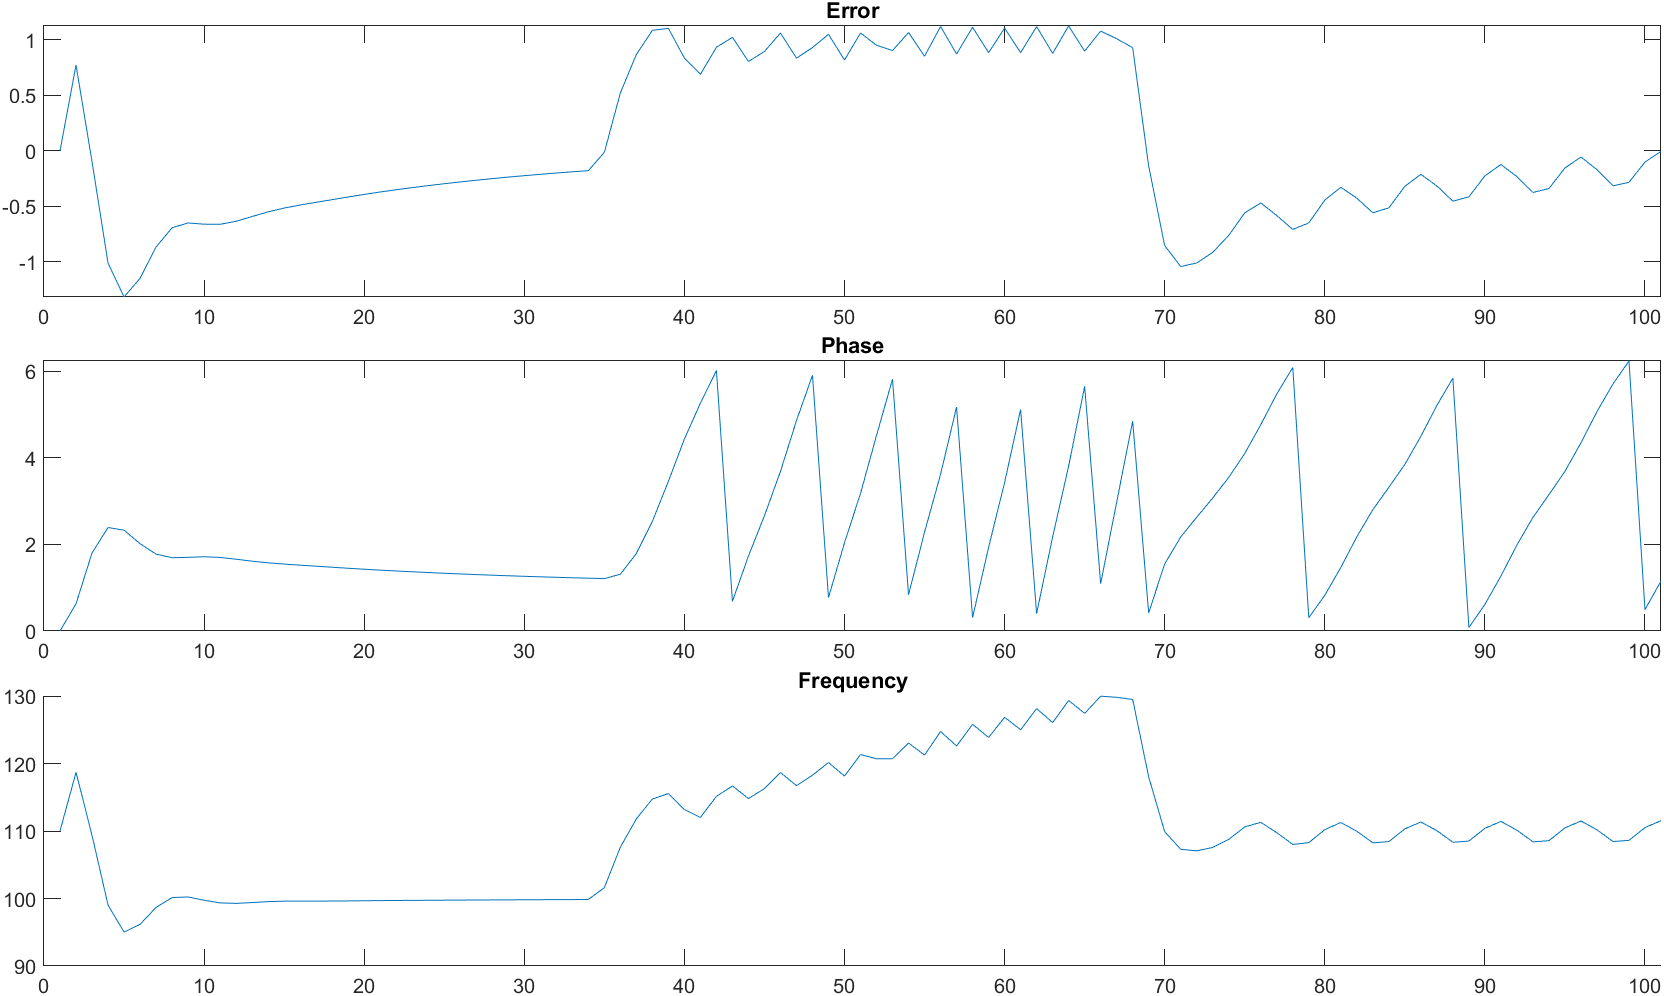
\includegraphics[width=0.7\textwidth]{p2_c.png}
    \end{subfigure}% 
    \\
    \begin{subfigure}{\textwidth}
      \centering
      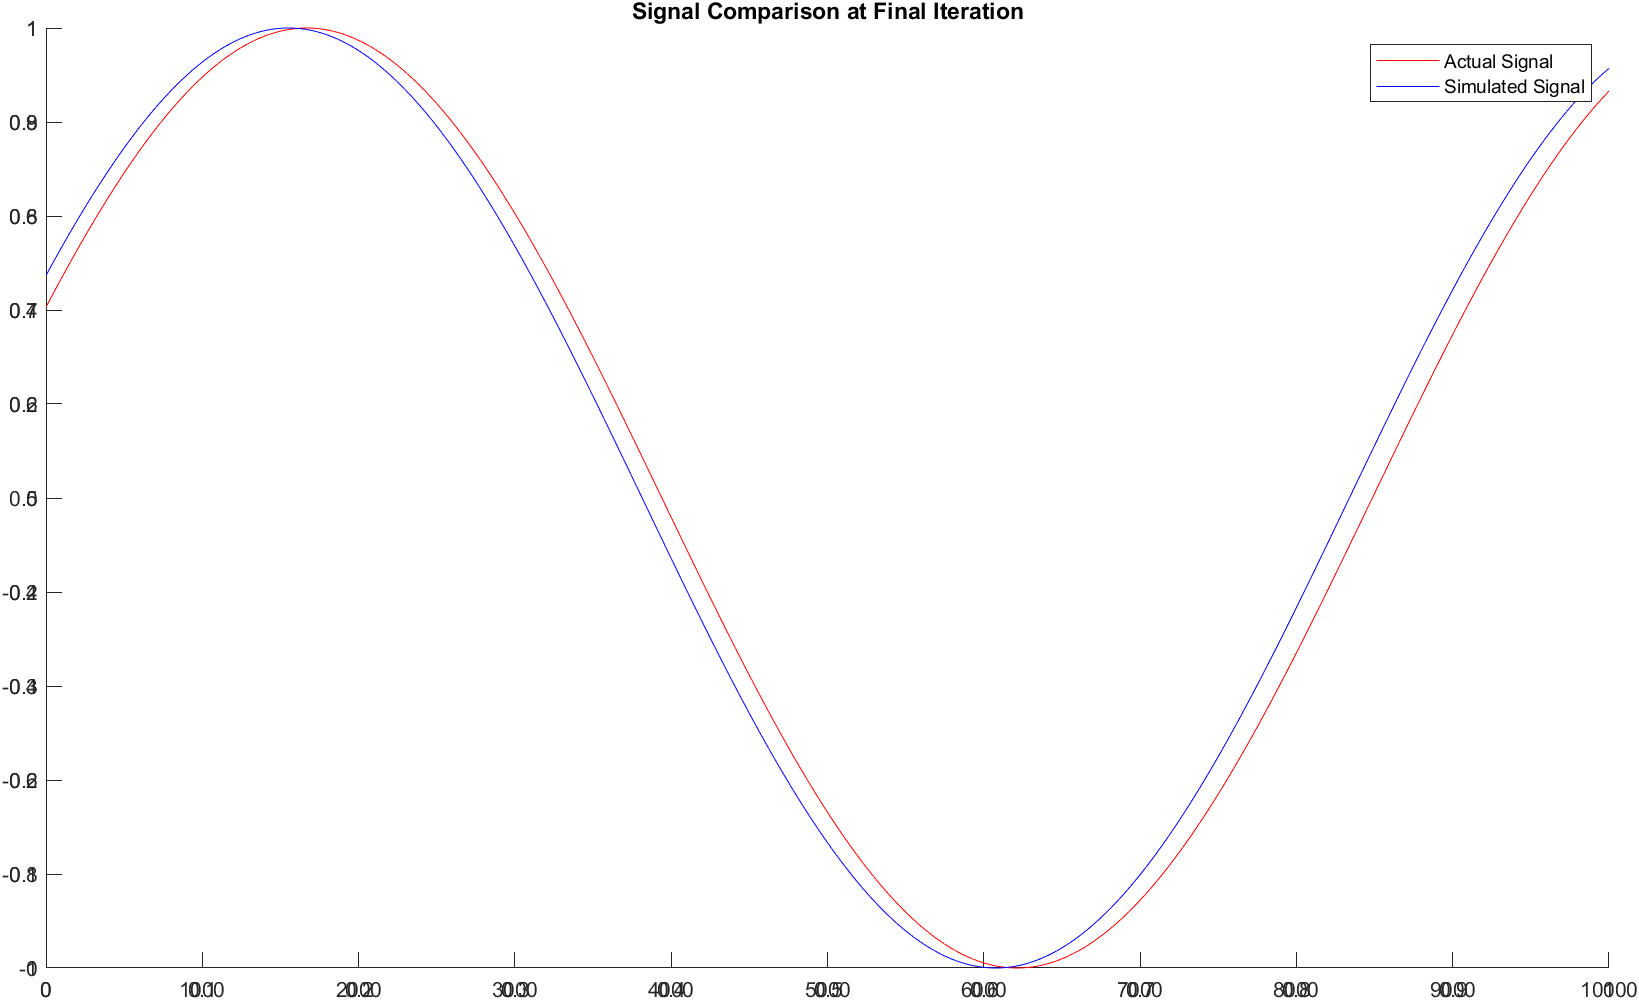
\includegraphics[width=0.7\textwidth]{p2_c_wave.png}
    \end{subfigure}%
    \caption{PLL Part C.}
    \label{fig:5}
  \end{figure}
  Lastly, assuming a nominal frequency of 10 Hz, the PLL designed in \emph{part 
  a} completely fails (\emph{Figure \ref{fig:6}}).
  \begin{figure}[H]
    \centering
    \begin{subfigure}{\textwidth}
      \centering
      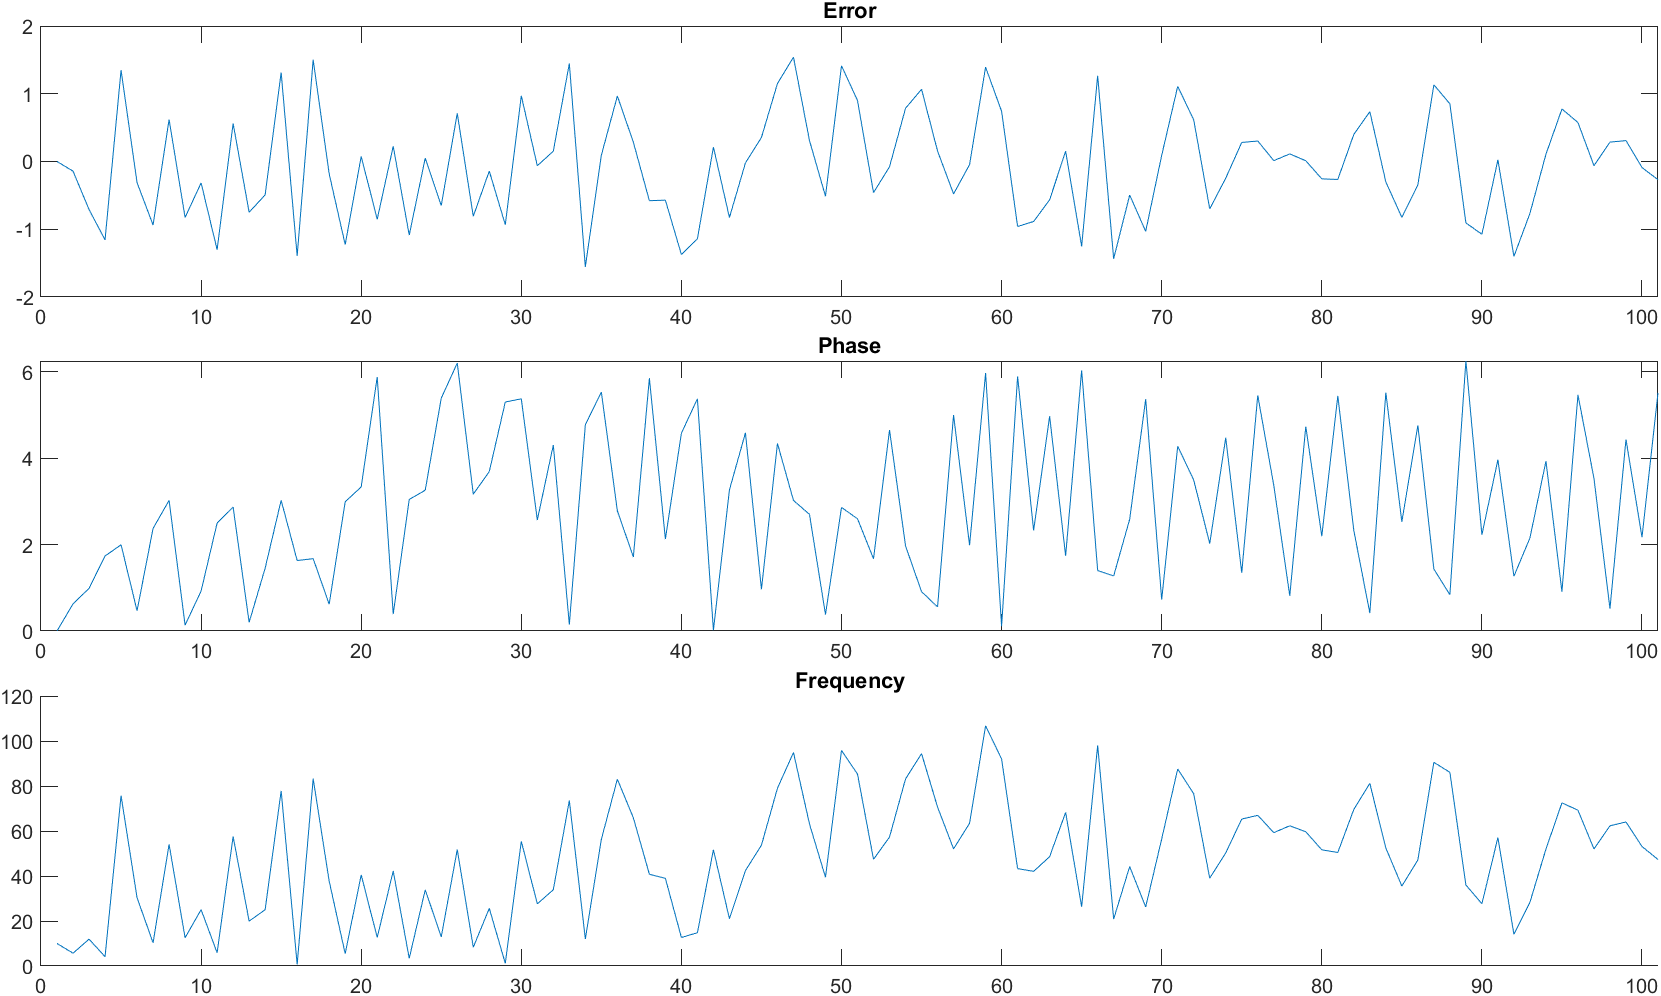
\includegraphics[width=0.7\textwidth]{p2_d.png}
    \end{subfigure}% 
    \\
    \begin{subfigure}{\textwidth}
      \centering
      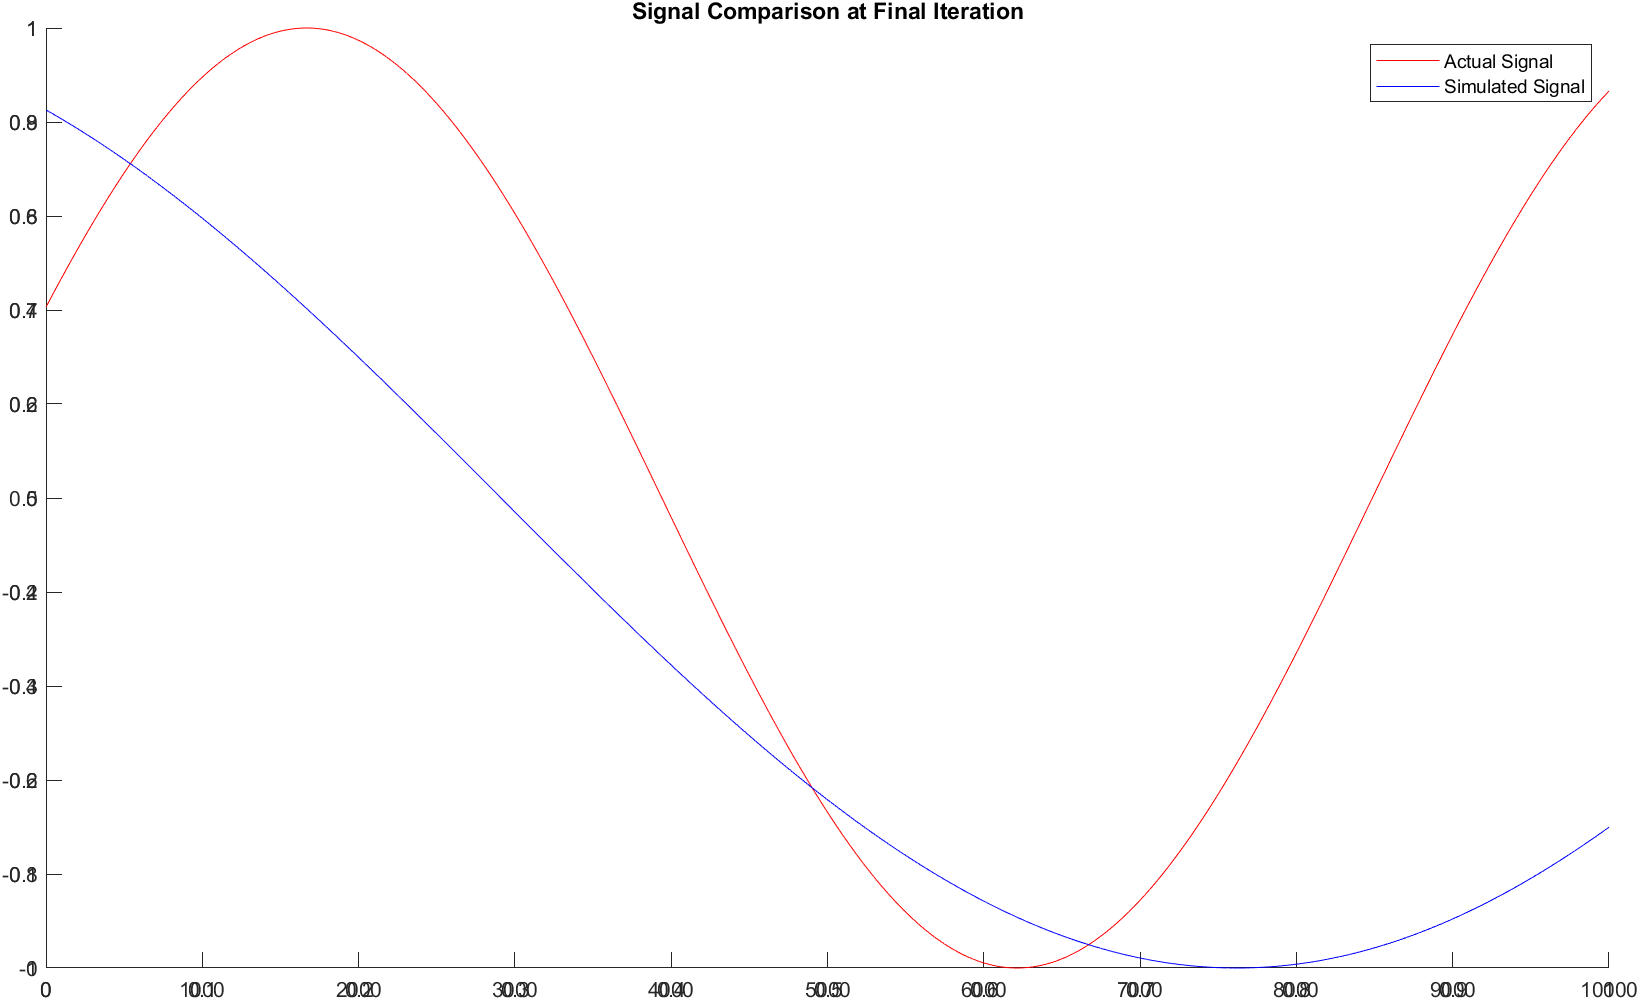
\includegraphics[width=0.7\textwidth]{p2_d_wave.png}
    \end{subfigure}%
    \caption{PLL Part D.}
    \label{fig:6}
  \end{figure}
  \vspace{12pt}


  % PROBLEM 3
  \item Modify your PLL from problem \#2 to operate as a Costas loop filter. Take 
  the 88 second data (generate\_signal(2)) sampled at 1 MHz and decode the data 
  message on the 100 Hz sinusoid using your Costas loop filter. The data bits 
  are 1 second wide and are comprised of 8 bit ascii characters. \\ \\
  \solution
  The same controller designed and discriminator used in \emph{Problem 2} was 
  used for the Costas Loop. The only addition was using of the "sign" of the 
  Inphase values as the values for the binary sequence. The resulting message 
  was "{\bf{AU WarEagle}}".
  \vspace{12pt}


  % PROBLEM 4
  \item Develop a simple DLL to phase align the sequence shown below with the 
  digital signal (generate\_signal(3)) provided on the website. The sequence is 
  sampled at 10 samples per chip. Plot the delay vs. time (or frequency vs. time 
  depending on your implementation).
  \begin{equation*}
    Sequence = \begin{bmatrix} 1 & -1 & -1 & -1 & 1 & -1 & 1 & 1 \end{bmatrix}
  \end{equation*} 
  \solution
  For this, a proportional only controller works well with $K_p = 5$. The 
  overall setup for a basic DLL is very similar to the PLL except it utilizes 
  a different discriminator. For 1/2 chip spacing, the discriminator is 
  $0.5\dfrac{E-L}{E+L}$. The following code was used for the DLL and 
  \emph{Figure \ref{fig:7}} shows the output.
  \begin{lstlisting}
  for i = 2:length(loop)
    % signal chunk
    sig = signal(beg:fin);
    % autocorrelatation
    E = correlation(sig, sequence, 'standard', tau(i-1)+s);
    L = correlation(sig, sequence, 'standard', tau(i-1)-s);
    % error
    disc(i) = 0.5 * (E-L)/(E+L);
    tau(i) = round(tau(i-1) + Kp*disc(i));
    beg = beg + 80;
    fin = fin + 80;
  end
  \end{lstlisting}
  \begin{figure}[H]
    \centering
    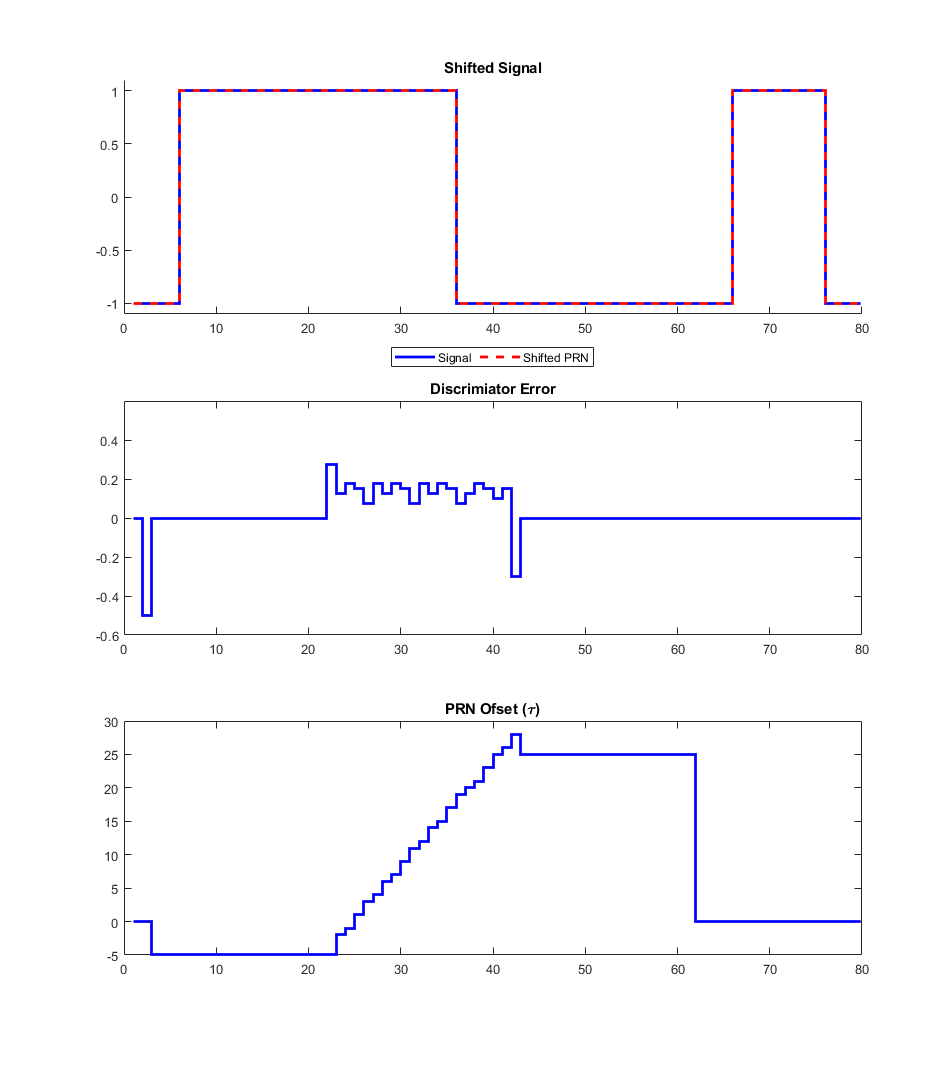
\includegraphics[width=0.7\textwidth]{p4_dll.png}
    \caption{Basic DLL.}
    \label{fig:7}
  \end{figure}
  \vspace{12pt}
  
  % PROBLEM 5
  \item Combine your Costas Loop filter from problem \#3 and your DLL from 
  problem \#4 to decode the data signal (generate\_signal(4)). \\ \\
  \solution
  \vspace{12pt}
  Signal 4 was incomplete, therefore this problem could not be completed.


  % PROBLEM 6
  \item Take the PRN code for SV \#4 or \#7 (i.e. from HW \#3) and upsample it 
  such that there are 16 samples at each chip (i.e. the length of this vector 
  will be 1023*16 long).
  \begin{enumerate}[(a)]
    \itemsep -2pt
    \item Show the autocorrelation calculation from -5 chips to +5 chips in 
    1/16 chip increments.
    \item Repeat with noise ($\sigma=0.2$) added to the non-shifted signal
  \end{enumerate}
  \solution
  For this problem, the PRN could be easily upsampled by an even number using 
  MATLAB's \emph{repelem} function. Running the autocorrelatation for this 
  upsampled PRN and an upsampled PRN with added noise results in \emph{Figure 
  \ref{fig:8}}. As shown, adding noise has visually no effect on the correlation 
  of the sequences proving even a noisy signal, like GPS, can be correlated 
  properly.
  \begin{figure}[H]
    \centering
    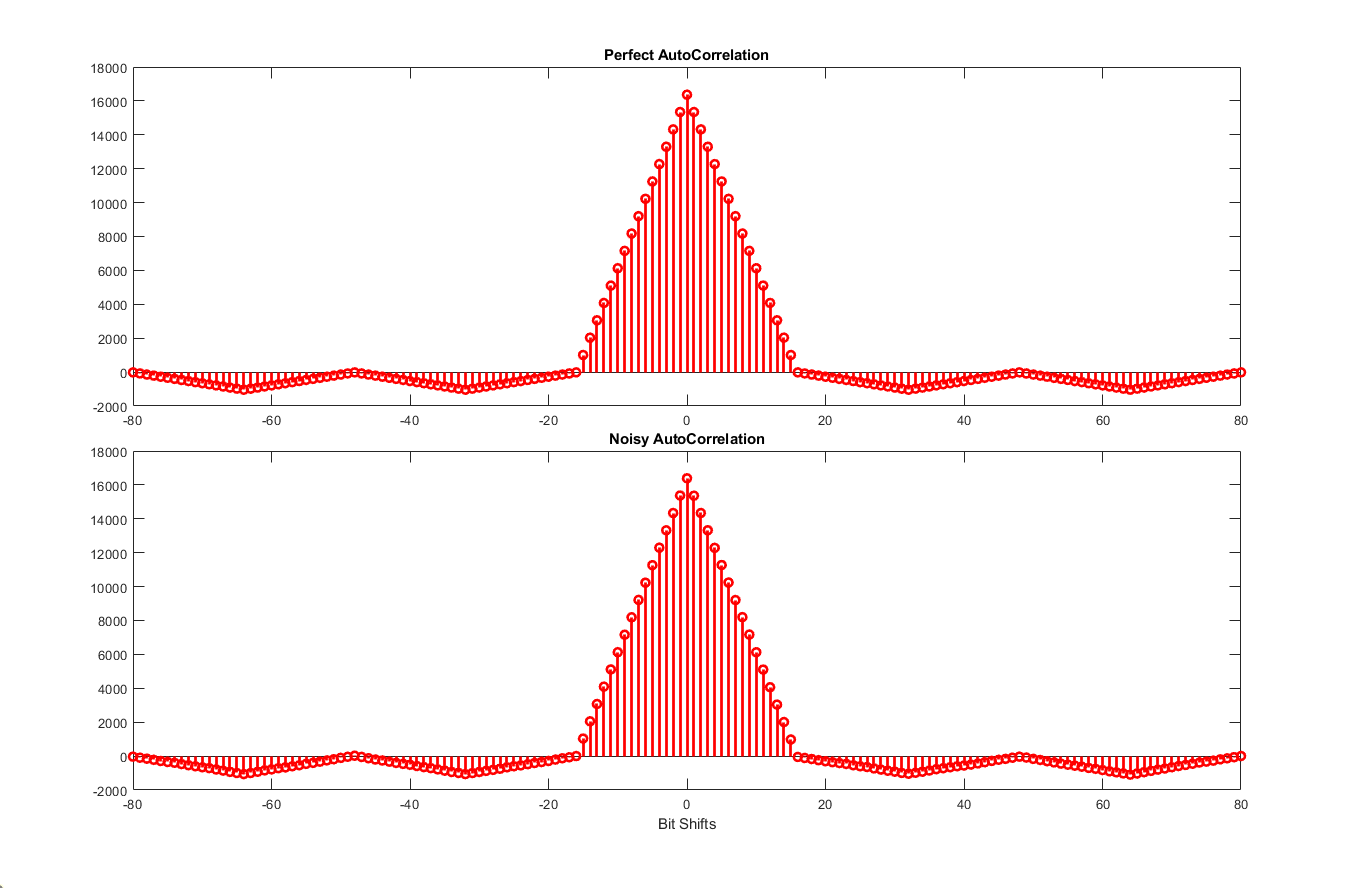
\includegraphics[width=0.9\textwidth]{p6_corr.png}
    \caption{Upsampled Autocorrelatation.}
    \label{fig:8}
  \end{figure}
  \vspace{12pt}


  % PROBLEM 7
  \item Write your own acquisition software to acquire a single satellite from 
  the IFEN IF data file. You can write a serial or parallel search algorithm. 
  Provide a plot of the acquisition plane (Code and Doppler) and provide the 
  code phase and Doppler results. The C/A (Gold) codes for several satellites 
  in view are on the website. \\
  \solution
  Using Tanner Watts's thesis, the technique for parallel satellite acquisition 
  was learned and utilized in the following code for satellite 7:
  \begin{lstlisting}
  idx = ceil(1/nSamples : 1023/nSamples : 1023-(1/nSamples));
  f_dopp = -10000:100:10000;
  [sig1, ~] = fread(fid, n_ms*nSamples, 'int8');
  % PRNS IN SEARCH
  for k = 1:32  
    prn_up = ca_code(k, idx)';
    % DOPPLER BINS
    for j = 1:length(f_dopp)
        % tanner watts's thesis
        f = f_if + f_dopp(j);
        I = sig1 .* sin(2*pi*f*t_samp);
        Q = sig1 .* cos(2*pi*f*t_samp);
        R1(:,j,k) = abs(ifft(fft(I + Q.*1j) .* conj(fft(prn_up)))).^2;
    end
  end
  \end{lstlisting}
  This PRN was acquired at a code shift of 989 (-34) chips and a doppler offset 
  of -500 Hz using only 1 ms of data. The acquisition plane is shown in 
  \emph{Figure \ref{fig:9}}. Using a 10 ms acquisition time results in a much 
  cleaner acquisition but still gets acquired at the same code and doppler 
  shifts (\emph{Figure \ref{fig:10}}). Interesting to note, over the 10 ms 
  acquisition period, 10 maximum peaks are observed at the same PRN offset in 
  each of the 10 replications of the PRN. Also iterating through all 32 
  satellites it can be determined that satellites {\bf{1}}, {\bf{7}}, {\bf{14}}, 
  {\bf{17}}, {\bf{19}}, {\bf{21}}, and {\bf{30}} are all in view after the first 
  1 ms of data.
  \newpage
  \begin{figure}[h]
    \centering
    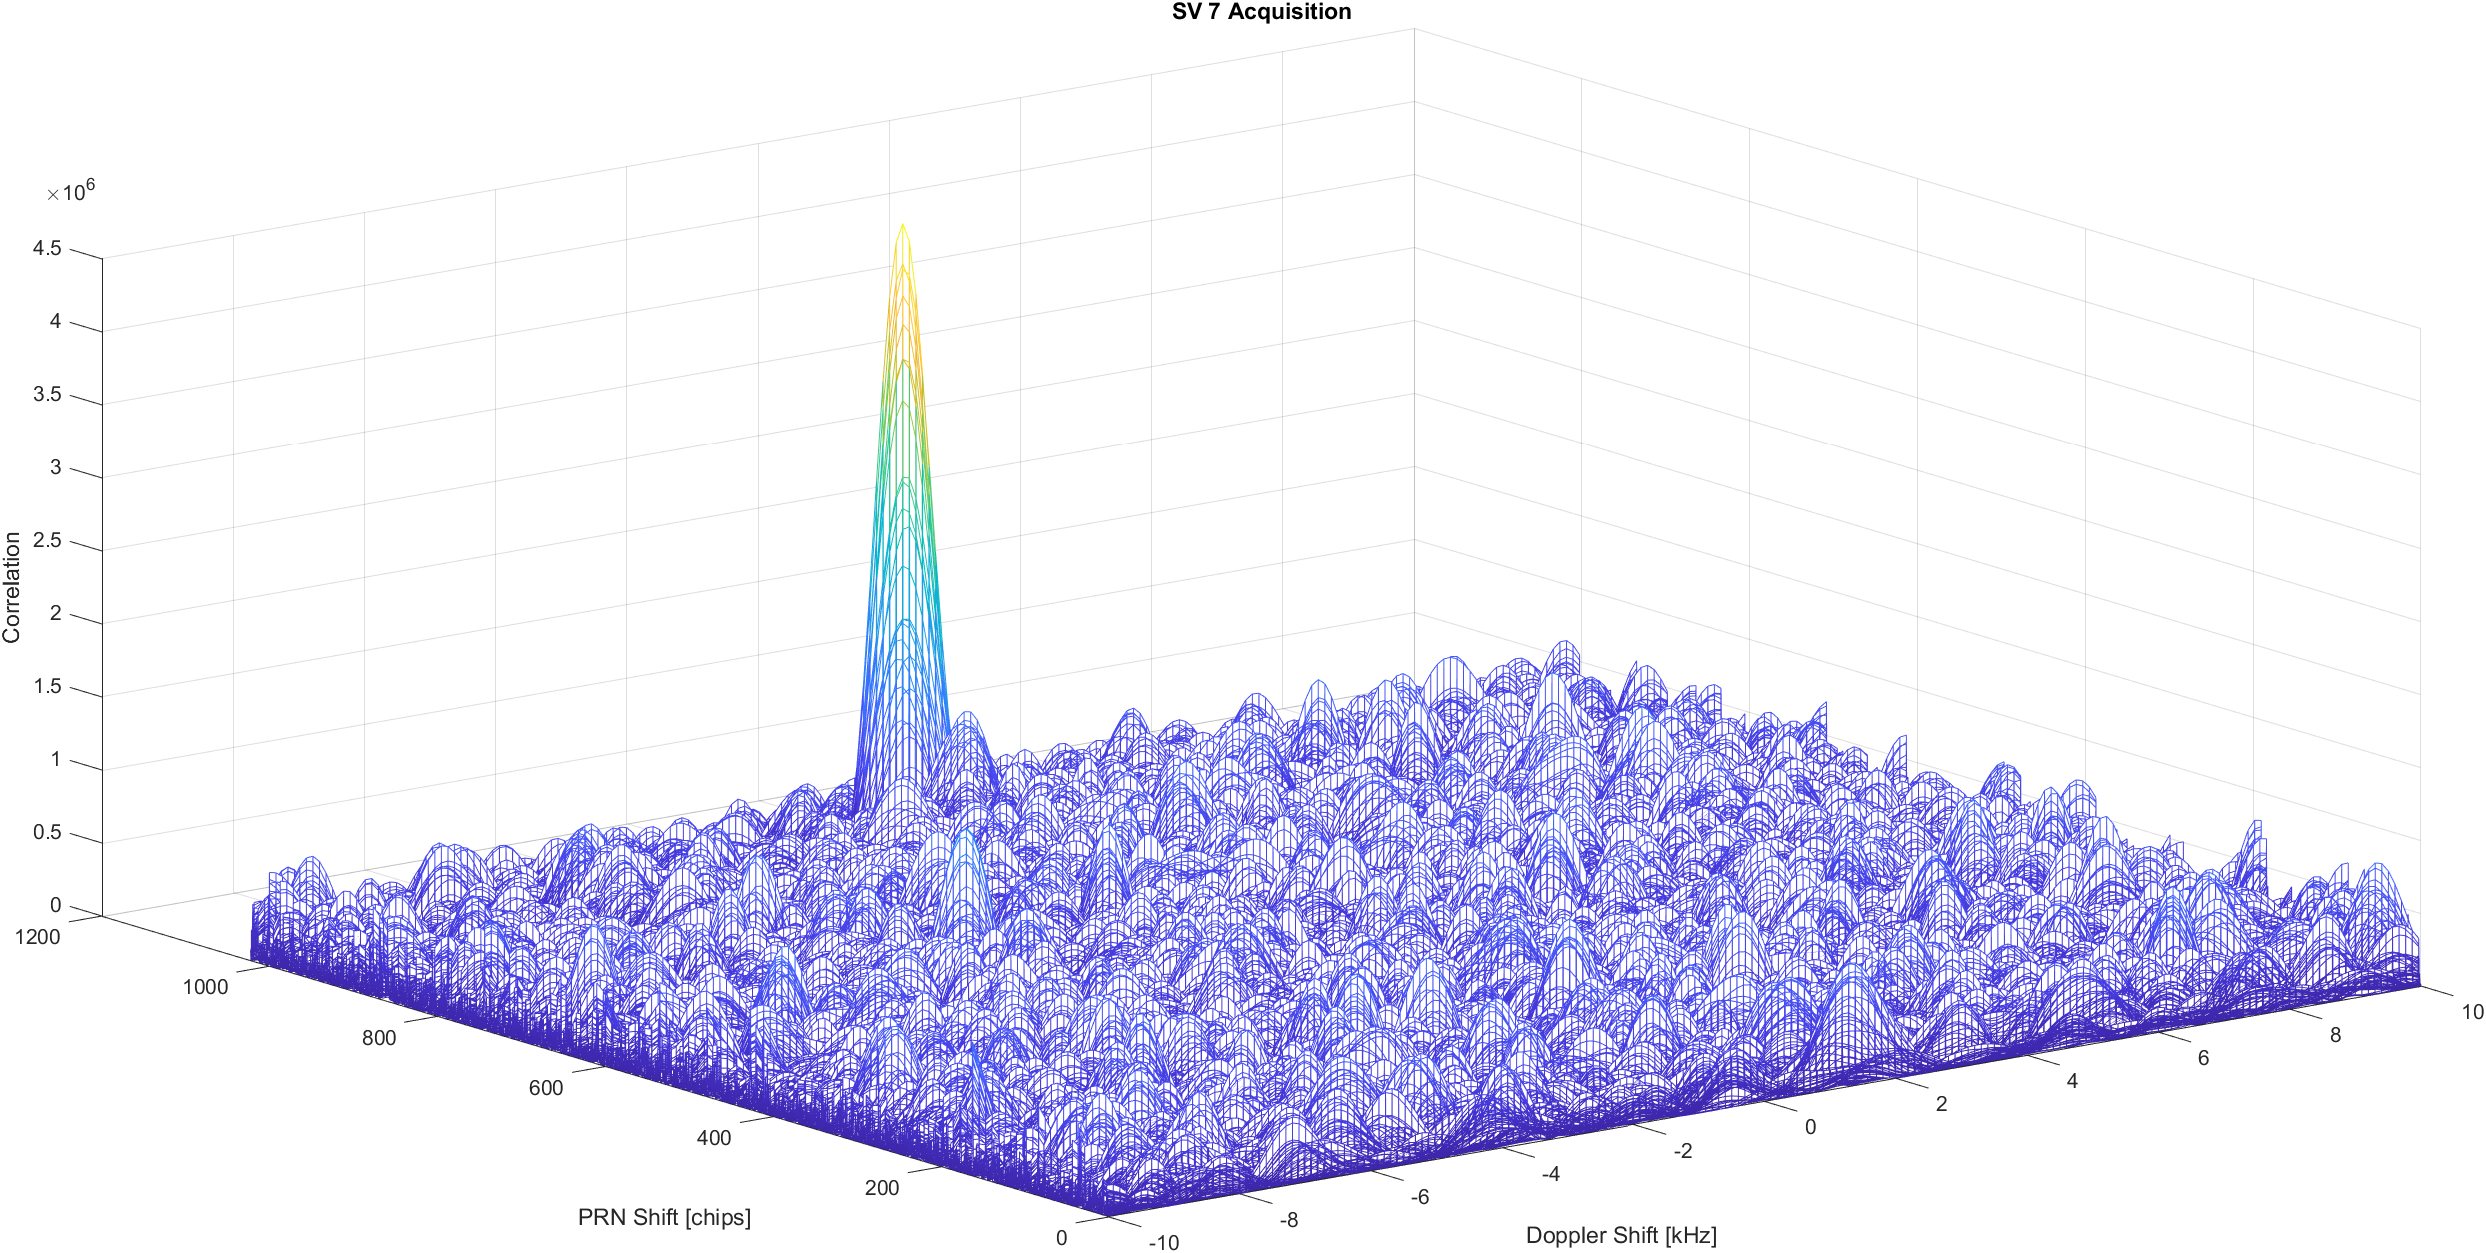
\includegraphics[width=0.8\textwidth]{p7_SV7.png}
    \caption{Satellite 7 Acquisition over 1 ms.}
    \label{fig:9}
  \end{figure}
  \begin{figure}[h]
    \centering
    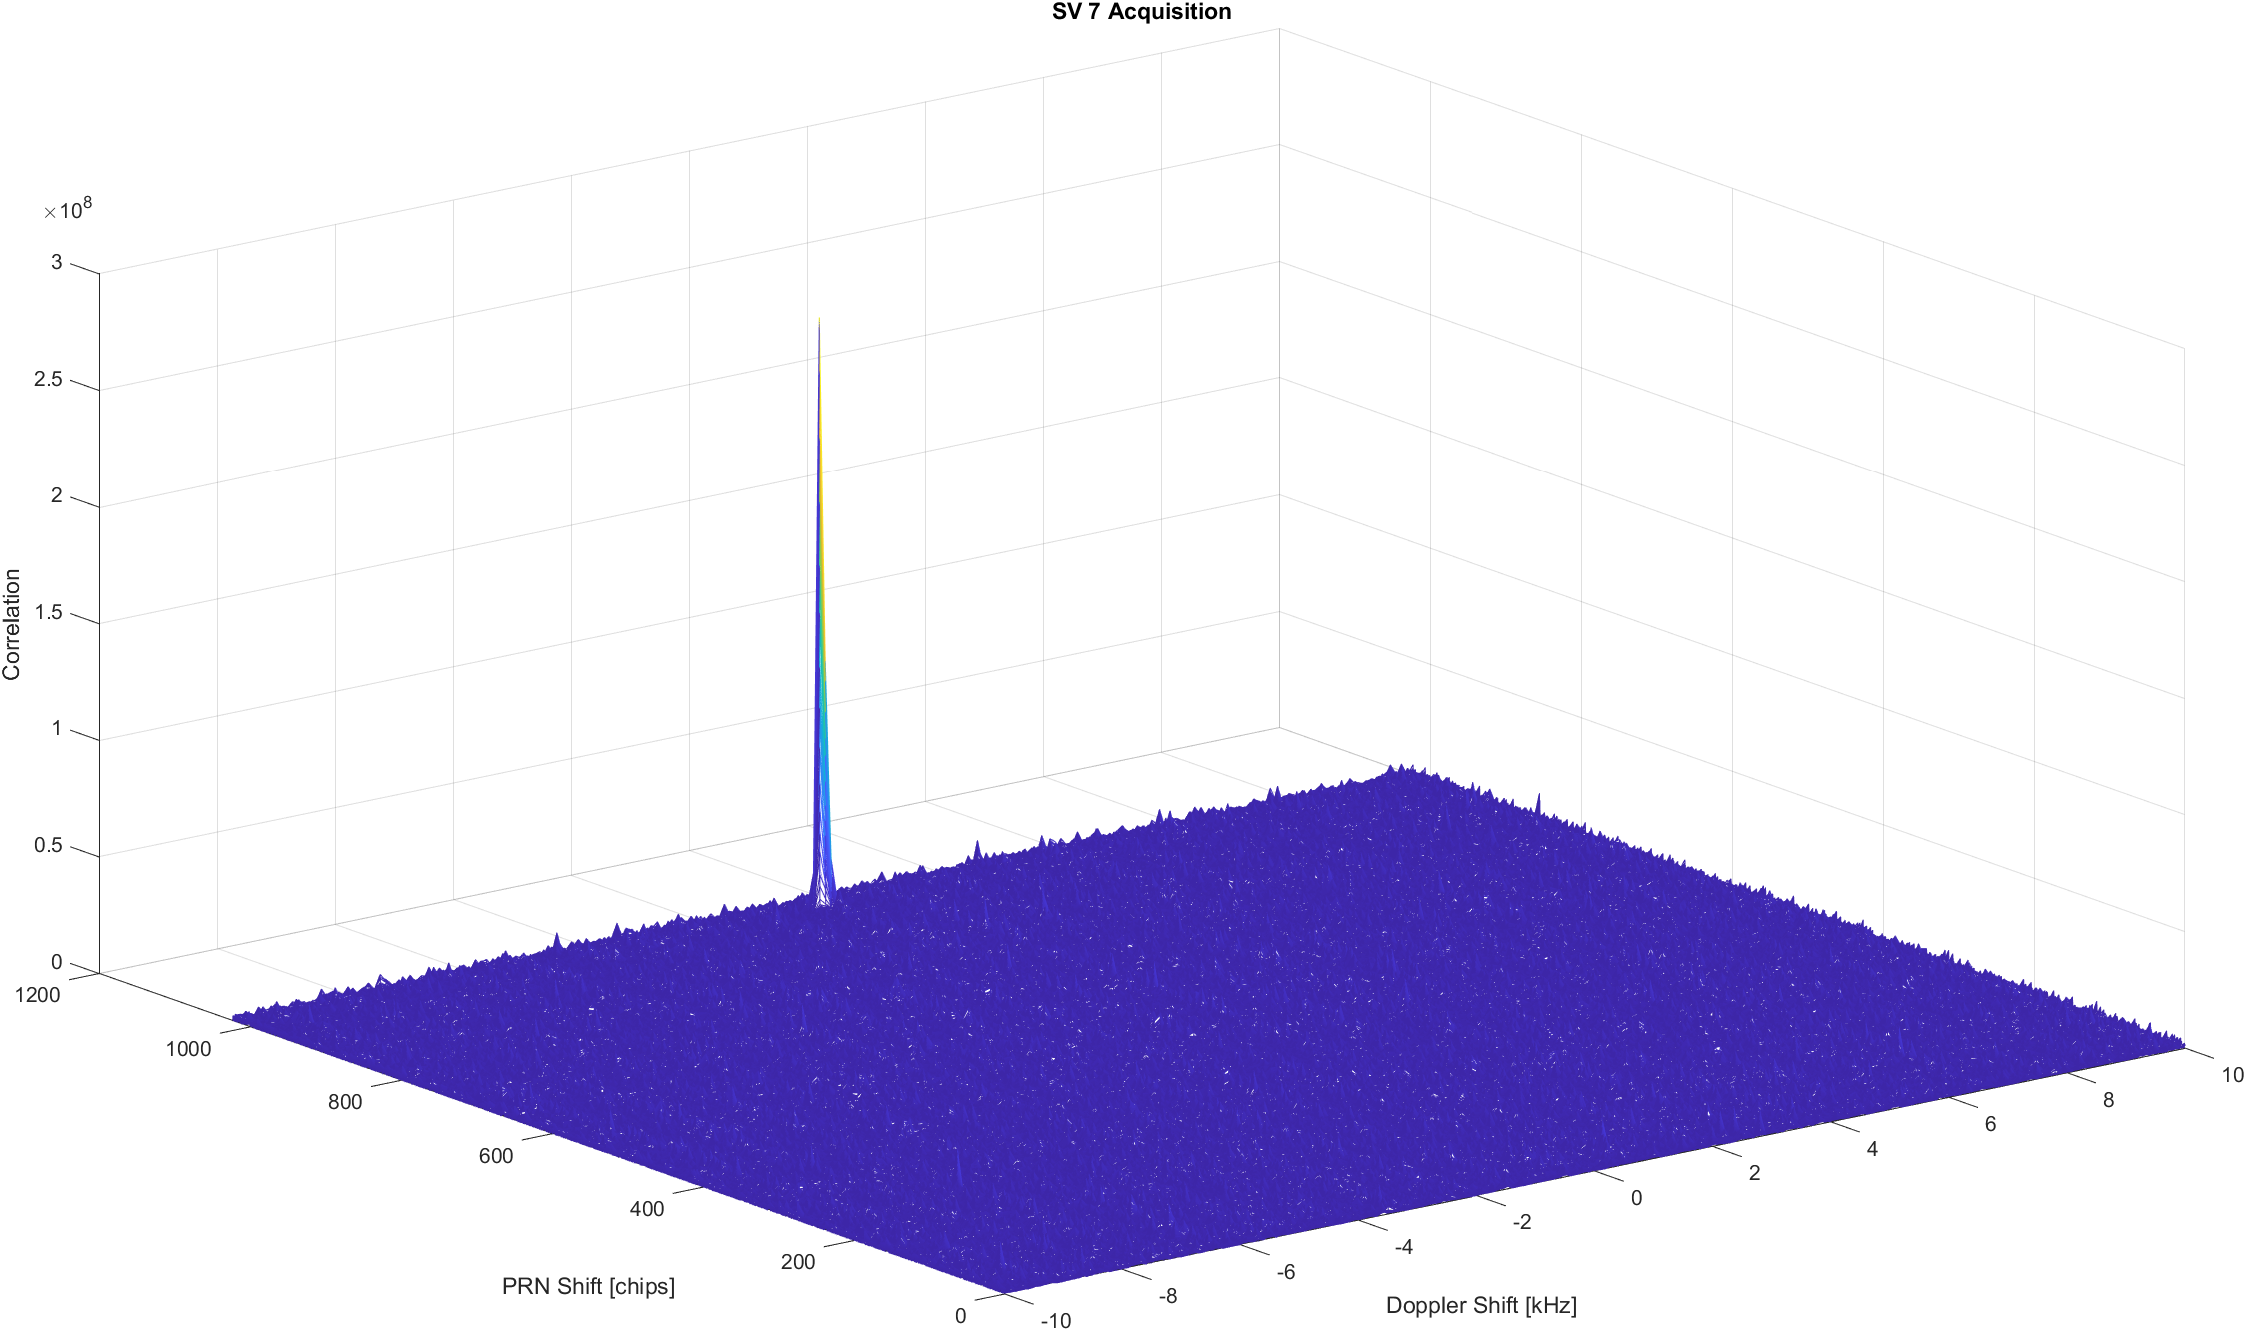
\includegraphics[width=0.8\textwidth]{p7_SV7_2.png}
    \caption{Satellite 7 Acquisition over 10 ms.}
    \label{fig:10}
  \end{figure}

\end{enumerate}

\end{document}